\section[Lehramtsstudium für Gymnasien \& Gesamtschulen (2-Fach-Bachelor)]{Lehramtsstudium für Gymnasien und Gesamtschulen (2-Fach-Bachelor)}
\begin{multicols*}{2}
An dieser Stelle soll der Ablauf des 2-Fach-Bachelors kurz erläutert werden. Dieser beinhaltet neben dem Fach Physik auch noch weitere Elemente wie euer Zweitfach und die Bildungswissenschaften.
\subsection*{Module}
Innerhalb des Studiums werden Vorlesungen, Übungen und Seminare in Modulen zusammen gefasst die dann in Modulabschlussprüfungen abgeschlossen werden. Die Noten dieser Prüfungen gehen alle in eure spätere Endnote mit ein. Eine Ausnahme stellen die Klausuren in Physik 1 bis 3 dar, hier wird die schlechteste Note gestrichen. Außerdem ist es leider nicht möglich die Modulabschlussprüfungen beliebig oft zu wiederholen, deswegen gibt es in den Klausuren in Physik 1 bis 3 vier Versuche und in allen weiteren nur drei.
\subsection*{Die Grundmodule}
In den ersten drei Semestern belegt ihr die grundlegenden Module für das Physikstudium: Dynamik der Teilchen und Teilchensysteme (Physik 1), Thermodynamik und Elektromagnetismus (Physik 2) und Wellen und Quanten (Physik 3). Physik 1 deckt sich im Prinzip mit dem Modul der 1-Fach-Bachelor, nur dass ihr noch ein spezielles Mathetutorium hört.In Physik 2 und Physik 3 hören die 1-Fach-Bachelor zusätzlich noch Theoretische Ergänzungen (TE). Zu den oben genannten jeweiligen Vorlesungen gibt es außerdem noch Übungen in denen ihn Aufgaben zu den Vorlesungen bekommt.\\ Im dritten und vierten Semester muss außerdem noch das Modul Experimentelle Übungen absolviert werden. Innerhalb dieses Moduls werdet ihr alle zwei Wochen eigene Experimente durchführen und dazu Versuchsberichte schreiben die bewertet werden.
\subsection*{Weitere Module}
Nach den oben genannten grundlegenden Modulen wird im vierten Semester das Modul Atom- und Quantenphysik absolviert. Dazu gehört die gleichnamige Vorlesung und Übung. In desem Modul werden ihr eure erste mündliche Abschlussprüfung von circa 30-45 Minuten haben.\\ Das fünfte Semester widmet sich dem Modul Struktur der Materie. Es beinhaltet Vorlesungen in Kern- und Teilchenphysik, Physik der kondensierten Materie und Astrophysik und Kosmoliogie. Allerdings müssen nur in den ersten beiden Übungen besucht werden. Auch dieses Modul wird durch eine mündliche Prüfung abgeschlossen.\\ Im sechsten Semester wird das Modul Messtechnik und Signalverarbeitung eineführt. Hier müsst ihr die Komibation aus Vorlesung und Übung in den Grundlagen der Signalverarbeitung absolvieren und durch eine mündliche Prüfung abschließen.\\ Des weiteren wird in den Semestern fünf und sechs das Modul Grundlagen der Fachdidaktik und Erkenntnistheorie absolviert. Es beinhaltet eine Vorlesung zur Einführung in die Fachdidaktik der Physik für das Lehramt Physik und ein Seminar zur Theorie, Geschichte und Kultur der Naturwissenschaften.\\ Am Ende könnt ihr euch entscheiden ob ihr eure Bachelorarbeit in der Physik oder in einem eurer anderen Fächer schreiben möchtet.
\subsection*{Bildungswissenschaften}
In den Bildungswissenschaften muss das Modul Einführung in Grundfragen von Erziehung und Bildung absolviert werden. Dazu gehören eine Vorlesung und ein frei wählbares Seminar. Es wird mit einer Klausur abgeschlossen. Außerdem muss das Eignungs- und Orientierungspraktikum abgeschlossen werden. Hierfür hospitiert ihr fünf Wochen in einer von euch gewählten Schule. Vor-und Nachbearbeitet wird das ganze in einem Seminar.Des weiteren gibt es noch das Berufsfeldpraktikum in dem ihr Berufsmöglichkeiten außerhalb des Lehramts kennen lernen sollt.

Das sind zunächst die wichtigsten Informationen die ihr für die Bewältigung eures Bachelorstudiums braucht. Solltet ihr noch weitere Fragen zum Bachelor oder vieleicht sogar schon zum Master haben könnt ihr gerne in die Fachschaft vorbei schauen. Dort hilft man euch gerne weiter. Bei grundlegenderen Fragen könnt ihr auch zu Zentralen Studienberatung gehen. Außerdem empfiehlt es sich natürlich die speziellen Infoveranstaltungen für Zwei-fach-bachelor während der Orientierungswoche zu besuchen :-)

\fibelsig{Andrea}

%\begin{center}
%	\fibelimgtext{
%		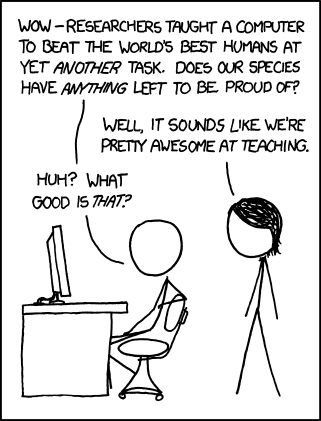
\includegraphics[width=\columnwidth, height=0.23\textheight]{res/xkcd/894_progeny.png}
%	}{\url{https://xkcd.com/894}}
%\end{center}
\end{multicols*}
